Results from experiments investigating the relationship between direct, indirect, and combined plasticity are reported in Sections \ref{sec:direct_result}, \ref{sec:indirect_result}, and \ref{sec:combined_result}.
To summarize, the emergence of gene regulatory networks exhibiting direct and indirect plasticity was observed in evolutionary trials where environmental influence on the phenotype exerted selective pressure for these traits.
Champion gene regulatory networks from evolutionary trials selecting for direct plasticity exhibited a higher incidence of silent mutation compared to champion gene regulatory networks evolved in control trials.
Champion gene regulatory networks from evolutionary trials selecting for indirect plasticity exhibited a higher incidence of phenotypically-expressed mutation and a lower incidence of silent mutation compared to champion gene regulatory networks evolved in control trials.
Both of these experimental treatments appear to leave the rate of lethal mutation unaffected.
Champion gene regulatory networks from evolutionary trials selecting for both indirect and direct plasticity exhibited a higher incidence of phenotypically expressed mutation.

\subsection{Direct Plasticity} \label{sec:direct_result}
The capacity of the gene regulatory networks modeled herein to exhibit direct plasticity --- the ability to consistently develop high-fitness phenotypes despite environmental noise --- was confirmed by comparison of the fitness achieved by champion individuals under exposure to environmental noise to a control group.
It was confirmed that champion individuals from the direct plasticity regime achieved fitness comparable to individuals evolved under a control regime.
Thus, it was concluded that the gene regulatory networks evolved were capable of coherent function despite some environmental noise.

Figure \ref{fig:es_direct} compares the evolvability signature of champion individuals evolved with and without environmental perturbation.
\begin{figure}
    \centering
    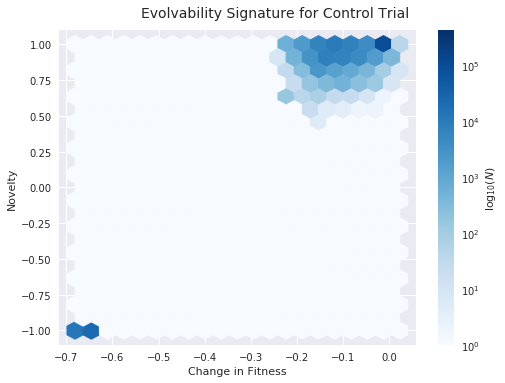
\includegraphics[width=0.5\textwidth]{img/es_p0} \\
    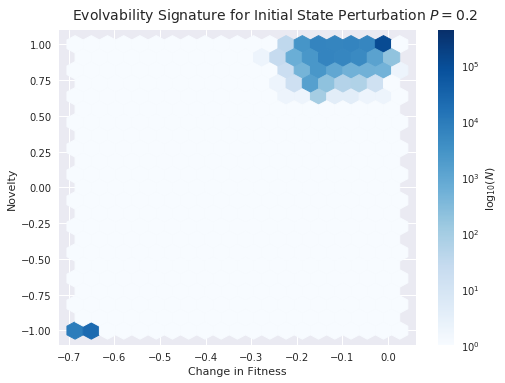
\includegraphics[width=0.5\textwidth]{img/es_p0_2}
\caption{Evolvability signatures of champion evolved without initial plasticity ($P = 0$) (top) and with initial plasticity ($P=0.2$). Figure after \cite{Tarapore2015EvolvabilityBenchmarks}.}
    \label{fig:es_direct}
\end{figure}
The evolvability signature co-visualizes the phenotypic and fitness outcomes of mutation.
Phenotypic novelty resulting from mutation, measured via the hamming distance between the phenotype expressed prior to and following mutation, is plotted on the $y$ axis.
Relative fitness of the phenotypes expressed prior to and following mutation is plotted on the $x$ axis.
The darkness of each tile represents the frequency of mutational outcomes that fall into that bin.
Silent mutations occur at the top right of the diagram, at the juncture of 0 novelty and 0 fitness consequence.
Lethal mutations are clustered at the bottom left of the evolvability signature.
Compared to the control evolvability signature, an overall reduction in the frequency of mutation with significant phenotypic and/or fitness consequences is observed under the direct plasticity regime.

This observation is accounted for in Figure \ref{fig:mutation_type_direct}, which compares the relative frequency with which silent, lethal, and phenotypically-expressed outcomes are observed from champion individuals evolved under the control and direct plasticity regimes.
\begin{figure}
    \centering
    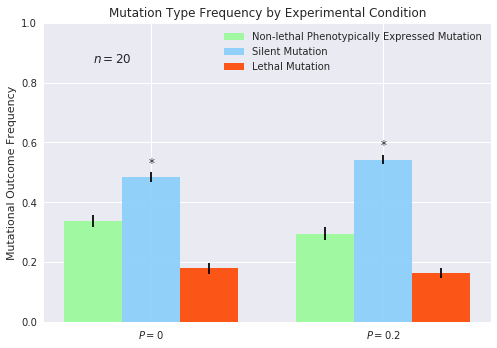
\includegraphics[width=0.5\textwidth]{img/mutation_type_direct}
  	\caption{Comparison of mutational outcome frequencies for champions evolved with and without initial state perturbation.}
    \label{fig:mutation_type_direct}
\end{figure}
A statistically significant increase in the incidence of silent mutation is observed under the direct plasticity regime.
This increase in the incidence of silent mutation appears to correspond to slight decreases in both the rates of lethal mutation and phenotypically expressed non-lethal mutation.

\subsection{Indirect Plasticity} \label{sec:indirect_result}
The capacity of the gene regulatory networks modeled herein to exhibit indirect plasticity --- the ability to simultaneously achieve high-fitness to a set of two of environmental condition/objective pairings --- was confirmed by comparison of the fitness scores for each environmental condition/objective pairing between champion individuals evolved with fitness determined exclusively via the primary condition/objective pairing and those evolved with fitness determined by both primary condition/objective pairings.
As expected, it was found that individuals exposed to the secondary condition/objective paring significantly outperformed individuals that were not with respect to that condition/objective pairing.
Champion individuals evolved exclusively to satisfy the primary condition/objective pairing exhibited statistically significant greater performance under the primary condition/objective pairing compared to individuals evolved to satisfy both condition/objective parings.
Nevertheless, the performance of champion individuals evolved to satisfy both condition/objective pairings at the primary condition/objective pairing was roughly comparable to that of champion individuals evolved exclusively to satisfy the primary condition/objective pairing; individuals evolved to satisfy both condition/objective pairings exhibited an obvious capacity to satisfy the primary condition/objective pairing.
These results are presented in Figure \ref{fig:primary_secondary_performance}.
It was concluded that the gene regulatory networks evolved in this model were capable of exhibiting indirect plasticity, simultaneously providing good performance on multiple condition/objective pairings.

\begin{figure}
    \centering
    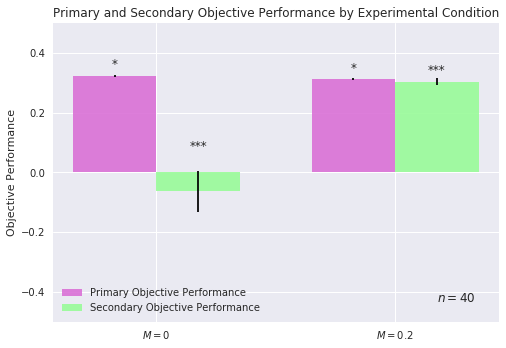
\includegraphics[width=0.5\textwidth]{img/primary_secondary_performance}
  	\caption{Comparison of objective performances of champions evolved with only primary condition/objective pair versus with both primary and secondary condition/objective pairs.}
    \label{fig:primary_secondary_performance}
\end{figure}

Figure \ref{fig:ev_indirect} compares evolvability visualizations of champion individuals evolved under control conditions, where selection took place exclusively for the primary condition/objective pairing, to individuals evolved to simultaneously satisfy both condition/objective pairings.
These visualizations were generated by measuring performance exclusively in terms of the primary condition/objective pairing.
These visualizations are comparable to the evolvability signatures provided in Figure \ref{fig:es_direct}, but track absolute fitness on the $x$ axis in lieu of relative fitness.
This change was made to ensure a clear comparison of the outcomes of mutation between champion individuals evolved exclusively under the control conditions, which enjoy slightly greater fitness in terms of the primary condition/objective pairing, and champion individuals evolved to simultaneously satisfy both condition/objective pairings.
A lower right hand region is outlined in red on these visualizations.
This region, the exact bounds of which were chosen arbitrarily, represents mutational outcomes in which mild fitness consequences are observed despite nontrivial phenotypic novelty.
Such mutational outcomes are desirable in terms of evolvability.
Preliminary analysis suggests that, despite overall relatively lower fitness of champion individuals, champion individuals evolved under an indirect plasticity regime more frequently generate mutational outcomes that fall into this region. 
More sophisticated statistical investigation would be necessary to confirm this finding.

\begin{figure}
    \centering
    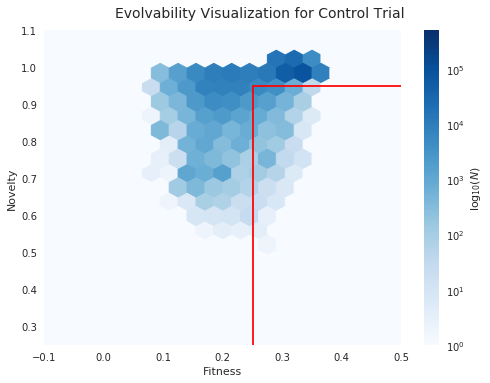
\includegraphics[width=0.5\textwidth]{img/ev_w0_target} \\
     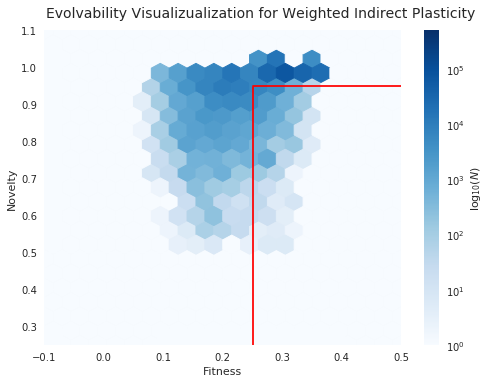
\includegraphics[width=0.5\textwidth]{img/ev_w0_2_target}
  	\caption{Evolvability visualization of champions evolved with only a primary condition/objective pair (top) and champions evolved with primary and secondary condition/objective pairs (bottom).}
    \label{fig:ev_indirect}
\end{figure}

Figure \ref{fig:mutation_type_indirect} compares the relative frequency with which silent, lethal, and phenotypically-expressed outcomes are observed from champion individuals evolved under control and indirect plasticity regimes.
It was found that evolution under the indirect plasticity regime induces a statistically-significant decrease in the frequency of silent mutation and a corresponding statistically-significant increase in the frequency of phenotypically-expressed non-lethal mutation.
The frequency of lethal mutation was not obviously affected.

\begin{figure}
    \centering
    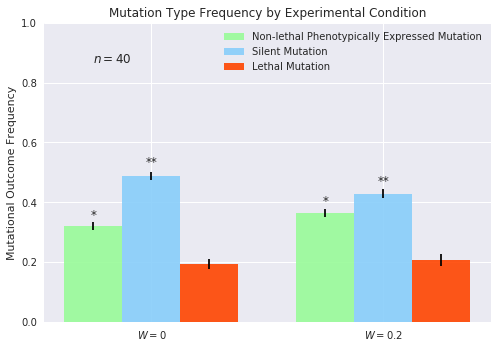
\includegraphics[width=0.5\textwidth]{img/mutation_type_indirect}
  	\caption{Comparison of mutational outcome frequencies for champions evolved with only primary condition/objective pair versus with both primary and secondary condition/objective pairs.}
    \label{fig:mutation_type_indirect}
\end{figure}

\subsection{Combined Plasticity} \label{sec:combined_result}
Similar to validation of the capacity of evolved gene regulatory networks to exhibit direct and indirect plasticity (reported in Sections \ref{sec:direct_result} and \ref{sec:indirect_result}), the capacity of evolved gene regulatory networks to exhibit both direct and indirect plasticity simultaneously was confirmed.
Specifically, it was found that champion individuals evolved under the combined plasticity regime exhibited comparable fitness relative to champion individuals evolved under the control regime in terms of the primary condition/objective pairing.
Figure \ref{fig:mutation_type_indirect} compares the relative frequency with which silent, lethal, and phenotypically-expressed outcomes are observed from champion individuals evolved under the control and combined plasticity regimes.
It was found that evolution under the combined plasticity regime induces a statistically-significant decrease in the frequency of silent mutation and a corresponding statistically-significant increase in the frequency of which phenotypically-expressed non-lethal mutation is observed.
Although not strong enough to merit statistical significance, this change in the frequency of phenotypically-expressed non-lethal mutation appeared to be accompanied by a corresponding decrease in both the frequency of silent mutation and the frequency of lethal mutation.

\begin{figure}
    \centering
    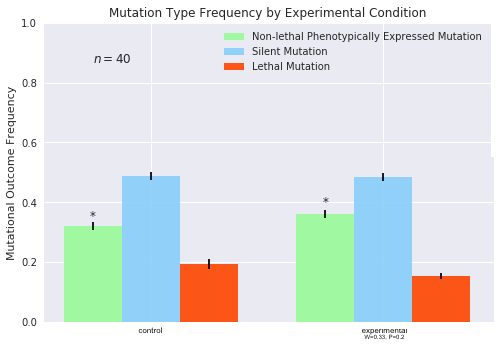
\includegraphics[width=0.5\textwidth]{img/mutation_type_combined}
  	\caption{Comparison of mutational outcome frequencies for champions evolved with only primary condition/objective pair and no initial state perturbation versus with both primary and secondary condition/objective pairs and initial state perturbation.}
    \label{fig:mutation_type_combined}
\end{figure}